% !TeX root = ../main.tex

\chapter{视频溯因常识推理}\label{cha:vacr}
本章会详细介绍视频溯因常识推理这个任务。第~\ref{sec:abductive}~节和第~\ref{sec:commonsense}~节中简单介绍了溯因推理和常识推理,第~\ref{sec:definition}~节中给出了视频溯因常识推理的定义。
\section{溯因推理}\label{sec:abductive}
溯因推理(Abductive Reasoning)是一种基于一些既定事实来推测原因的一类推理。在第~\ref{sec:visural_reasoning}~,我们已经介绍了$\alpha$NLI\cite{bhagavatula2019abductive}。$\alpha$NLI 是一个基于自然语言的溯因推理任务,在这里再次明确一下溯因推理的定义。为了降低难度,这里将溯因推理任务定义成多选一的选择题否则若要求模型自主生成假设将会更加困难。溯因推理包括以下几个部分:
\begin{enumerate}
    \item 观测:$O_1$和$O_2$,用来表示开始状态和结束状态。
    \item 假设:集合$\gH=\{H_i\}=\{H_+\}\bigcup\gH_{-}$。其中$H_+$表示正确选项,$\gH_-$表示所有的错误选项。
\end{enumerate}
模型需要根据两个观测$O_1$和$O_2$来从假设集合$\gH$中选出正确的选项。从概率模型的角度\cite{bhagavatula2019abductive},可以得到:
\begin{equation}
    H^{*}=\argmax _{H^{i}} P(H_+=H_i | O_{1}, O_{2}).
    \label{equ:prob}
\end{equation}
其中$H^*$为模型预测的最佳假设,$P(H_+=H_i|O_1, O_2)$表示在已知$O_1$和$O_2$的情况下,模型预测$H_i$为正确选项的概率。式~\eqref{equ:prob}~可以做如下变形:
\begin{equation}
    \begin{split}
        P(H_+=H_i | O_{1}, O_{2}) &= \frac{P(H_+=H_i, O_1, O_2)}{P(O_{1}, O_{2})} \\
        &= \frac{P(O_2|H_+=H_i, O_1)P(H_+=H_i|O_1)P(O_1)}{P(O_{1}, O_{2})}\\
        &\propto P(O_2|H_+=H_i, O_1)P(H_+=H_i|O_1)。
    \end{split}
    \label{equ:prob_model}
\end{equation}
其中最后一行是因为$P(O_1, O_2)$和$P(O_1)$与$H_i$无关。由此,我们可以得到图~\ref{fig:prob_model}~所示的五种概率模型:
\begin{enumerate}
    \item 仅假设($H$):若事件$H_+=H_i$与$O_1$和$O_2$都独立,则有
    \begin{equation}
        P(H_+=H_i | O_{1}, O_{2})\propto  P(H_+=H_i).
    \end{equation}
    \item 假设和第一个观测($H+O_1$):若事件$H_+=H_i$与$O_2$独立,则有
    \begin{equation}
        P(H_+=H_i | O_{1}, O_{2})\propto  P(H_+=H_i|O_1).
    \end{equation}
    \item 假设和第二个观测($H+O_2$):若事件$H_+=H_i$与$O_1$独立,则有
    \begin{equation}
        P(H_+=H_i | O_{1}, O_{2})\propto  P(H_+=H_i|O_2).
    \end{equation}
    \item 线性链(Linear Chain, LC):若$O_1$和$O_2$独立,则
    \begin{equation}
        P(H_+=H_i | O_{1}, O_{2})\propto  P(O_2|H_+=H_i)P(H_+=H_i|O_1).
        \label{equ:LC}
    \end{equation}
    \item 全连接(Fully Connected, FC):最普遍的情况,与式~\eqref{equ:prob_model}~一致。
\end{enumerate}
\begin{figure}[t]
    \def\firstwidth{.31\textwidth}
    \def\secondwidth{.46\textwidth}
    \centering
    \begin{subfigure}{\firstwidth}
        \includegraphics[width=\textwidth,page=1]{abduct1.pdf}
        \caption{仅假设}
    \end{subfigure}\hfill%
    \begin{subfigure}{\firstwidth}
        \includegraphics[width=\textwidth,page=2]{abduct1.pdf}
        \caption{假设和第一个观测}
    \end{subfigure}\hfill%
    \begin{subfigure}{\firstwidth}
        \includegraphics[width=\textwidth,page=3]{abduct1.pdf}
        \caption{假设和第二个观测}
    \end{subfigure}\\[2em]
    \begin{subfigure}{\secondwidth}
        \includegraphics[width=\textwidth,page=1]{abduct2.pdf}
        \caption{线性链}
    \end{subfigure}\hfill
    \begin{subfigure}{\secondwidth}
        \includegraphics[width=\textwidth,page=2]{abduct2.pdf}
        \caption{全连接}
    \end{subfigure}
    \caption{溯因推理的概率模型}
    \label{fig:prob_model}
\end{figure}
这些概率模型给出了在不同条件下来预测$H^*$的表达式。在这些概率模型中,只有全连接模型充分地考虑了各种已知信息的联系,其他的模型或是没有利用完整的观测信息($H$,$H+O_1$,$H+O_2$),或是仅仅分别考虑假设与两个观测的依赖关系(LC)。对于一个好的溯因推理任务,全连接的概率模型(FC)的推理表现应该比其他几种都要高,否则则说明这个推理任务的正确答案对两个观测$O_1$和$O_2$的依赖性不强。所以在之后的实验中,可以用这些概率模型来检验本文提出的视频溯因常识推理任务以及及数据集VideoABC。

\section{常识推理}\label{sec:commonsense}
常识推理(Commonsense Reasoning)顾名思义,是一类在推理过程中需要一些基本常识的推理任务。例如在Zellers~\etal 提出的视觉常识推理\cite{zellers2019recognition}任务中,模型需要通过选择题的形式来回答一些和常识有关的问题,并给出一个做出这个选择的原因。这个任务中的图片来自于影视片段,所以包含大量的人类日常生活中的场景。衡量一个任务是否具有常识性的最简单的方法就是让人类亲自尝试这个任务,并体会在推理的过程中是否用到了常识。从这个的角度来看,教程类视频比较适合来构建和常识推理相关的任务。教程类视频中具有明确的主题和步骤,所以人类能够很容易就可以理解视频的内容,并在多数情况下可以结合生活中的常识判断出不同步骤之间的时序关系。例如在买地铁票的视频中,人类甚至不用看到视频的题目,只需要看到售票机就可知道这个视频是在介绍如何买地铁票,并可以根据常识来回忆出买地铁票的步骤。

\section{视频溯因常识推理}\label{sec:definition}

在本节中,我们明确给出视频溯因常识推理任务的定义。视频溯因常识推理构建在溯因推理的架构上(详见第~\ref{sec:abductive}~节)。具体来说,该任务中的观测和假设的构成如下:
\begin{enumerate}
    \item $O_1$和$O_2$分别为一个完整推理过程的开始状态和结束状态的图片;
    \item $\gH=\{H_i\}$为候选的假设集合,其中每个$H_i$由多个视频构成,每个视频代表一个步骤。即
    \begin{equation}
        H_i = \{v_{i1}, v_{i2}, \ldots, v_{il_i}\},
    \end{equation}
    其中$v_{ij}$表示第$i$个假设中第$j$个步骤,$l_i$表示第$i$个假设中的步骤个数。
\end{enumerate}
模型需要根据两个观测信息来从假设集合$\gH$中选出正确的选项。该任务具有以下几个特点:
\begin{enumerate}
    \item 模型的输入只包含视觉信息。与之前视觉问答相关的任务不同,本文提出的\VACR 中没有任何自然语言的输入。也就是说,模型不会从自然语言中直接或间接获取到推理的过程,从而必须自己学会推理的过程。
    \item 复杂的视觉信息。任务中包含的视觉信息都来自于真实世界的图片或视频,包括人类日常生活中的各种复杂的任务,从而需要模型学会理解一些常识。
    \item 明显的时序关系。每一个假设$H_i$中的步骤都具有明显的时序关系。为了取得较好的推理效果,模型需要能够对步骤内和步骤间的时序关系建模。
\end{enumerate}


\begin{figure}
    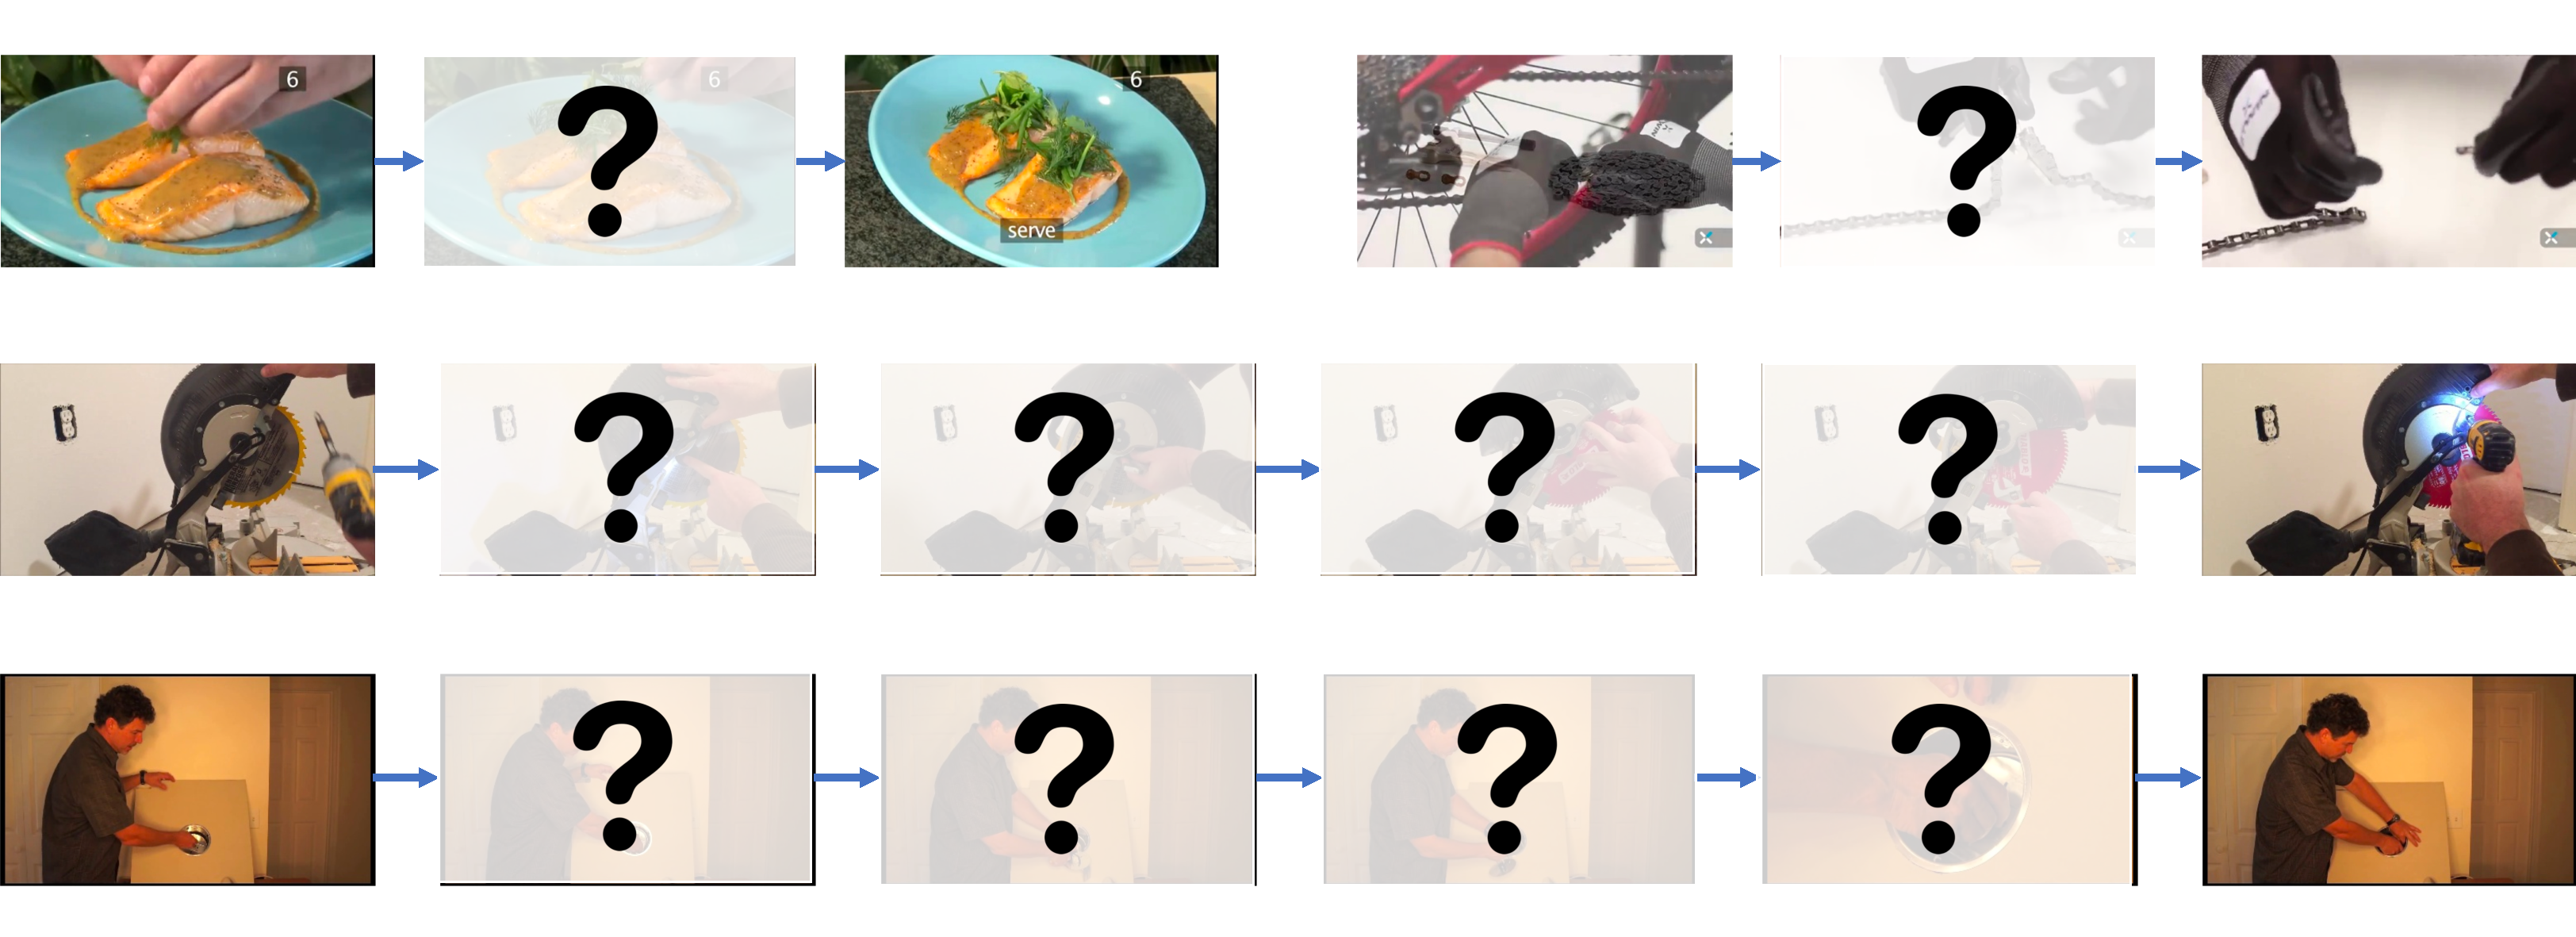
\includegraphics[width=\textwidth]{demo.pdf}
    \caption{视频溯因常识推理}
    \label{fig:vacr}
\end{figure}
图~\ref{fig:vacr}~展示了\VACR 的一些例子,包含了四种不同的任务可以看到,每个任务中用的已知条件只有开始和结束的两张图片,而中间的步骤是未知的。模型就是要从这两张已知的图片中选出最合适的步骤序列。同时也可以看到,这里的步骤数目是不确定的。因此,模型必须能够具有处理变长度步骤序列的能力才可以在该任务上取得比较好的表现。

由于\VACR 任务是一个建立在真实视觉信息上的推理任务,未来可能具有许多潜在的应用。例如,该任务可能会应用在机器人的决策问题中,尤其是哪些需要与真实世界具有频繁交互的决策任务。机器人首先可以拍照获取初始状态,用户可以给机器人输入一个目标状态,机器人通过搜索的方法可以得到很多种执行步骤。如果机器人可以顺利地完成\VACR 任务,那么它就可以从这些候选步骤序列中选出正确的一个,从而完成决策。
